\section{Adversarial Attacks}\label{chap:state-of-the-art}

Many machine learning models, including neural networks, consistently
misclassify adversarial examples - inputs formed by applying small but
intentionally worst-case perturbations to examples from the dataset, such that
the perturbed input results in the model outputting an incorrect answer with
high confidence \cite{goodfellow2014explaining}. An adversarial example is
described as

\begin{equation}
    \vect{x}^{adv}  = \vect{x} + \vect{\eta}.
\end{equation}

Where $\vect{x}^{adv}$ is the adversarial example, $x$ the original input and $\eta$
the perturbation.


First, this section describes the most promiment methods (attacks) to generate
adversarial examples and then highlights efforts that have been made to connect
adversarial examples with autoencoders. The attacks mentioned here can be found
in the cleverhans\footnote{github.com/tensorflow/cleverhans} library.
Contributions to the library in relation with this paper can be found here\footnote{github.com/tensorflow/cleverhans/pull/1037}
and here\footnote{github.com/tensorflow/cleverhans/pull/1047}.

\subsection{Fast Gradient Sign Method}
The "fast gradient sign method" (FGSM) refers to an attack that computes the
perturbation $\eta$ by calculating:

\begin{equation}\label{eq:fgsm}
    \vect{\eta} = \epsilon * sign(\nabla_x J (\vect{\theta}, \vect{x}, y)).
\end{equation}

Where $\vect{\theta}$ are the parameters of a model, $\vect{x}$ the input to the
model, $y$ the targets associated with $\vect{x}$ (for machine learning tasks
that have targets) and $J(\vect{\theta}, \vect{x}, y)$ the loss used to train
the neural network. Equation \ref{eq:fgsm} linearizes the cost function around
the current value of $\vect{\theta}$, obtaining an optimal max-norm constrained
pertubation $\vect{\eta}$. The elements of $\vect{\eta}$ are equal to the sign of
the elements of the gradient of the loss function with respect to the input.
$\epsilon$ is a number big enough such that the adversarial example is
effective, but small enough such that it won't be noticed in the generated
example. Figure \ref{fig:fgsm_panda} \cite{goodfellow2014explaining} visualizes
the effect of FGSM.


\begin{figure}
	\centering
	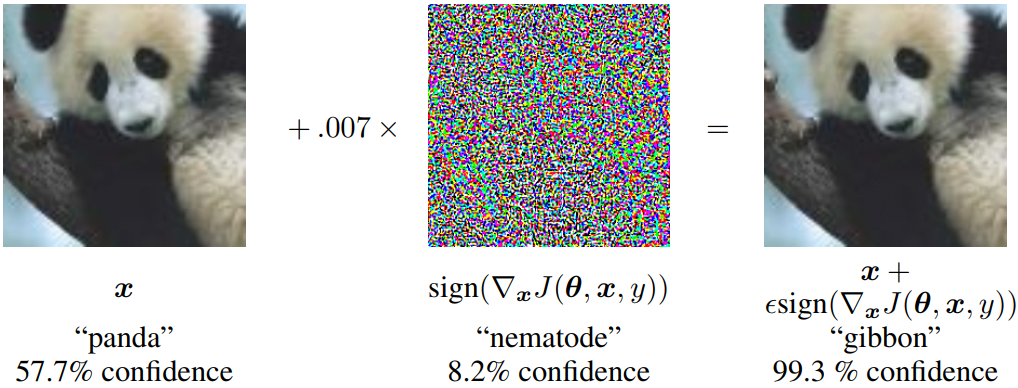
\includegraphics[width=\linewidth]{/3/fgsm_panda}
    \caption{FGSM applied to GoogLeNet \cite{szegedy2015going} on ImageNet. By
    adding an inconspicuous pertubation to the original image, GoogLeNet's
    classification of the image can be changed.} 
	\label{fig:fgsm_panda}
\end{figure}

\subsection{Projected Gradient Descent}
A straightforward way to enhance FGSM is, to apply it multiple times with a
small step size, and clip pixel values of intermediate results after each step
to make sure that they are in an $\epsilon-neighbourhood$  of the original
image:


\begin{equation}\label{eq:fgsm}
    \vect{x}^{adv}_{0} = \vect{x}, \quad \vect{x}^{adv}_{N + 1}=Clip_{x, \epsilon} \Big \{\vect{x}^{adv}_{N} + \alpha sign\big(\nabla_{x}J(\vect{x}^{adv}_{N}, y)\big)  \Big\}
\end{equation}

Typcially $\alpha = 1$ is used. This means that value of each poxel is only
changed by 1 on each step. This method is known as "projected gradient descent"
(PGD) or "basic iterative method". \cite{kurakin2016adversarial, madry2017towards}